\clearpage

\lehead[]{\sf\hspace*{-2.00cm}\textcolor{white}{\colorbox{lightblue}{\makebox[1.60cm][r]{\thechapter}}}\hspace{0.17cm}\textcolor{lightblue}{\chaptertitle}}
\rohead[]{\textcolor{lightblue}{\chaptertitle}\sf\hspace*{0.17cm}\textcolor{white}{\colorbox{lightblue}{\makebox[1.60cm][l]{\thechapter}}}\hspace{-2.00cm}}
%\chead[]{}
\rehead[]{\textcolor{lightblue}{AvHG, Inf, My}}
\lohead[]{\textcolor{lightblue}{AvHG, Inf, My}}

\section{Cartoon: How Projects Really Work}

\bgroup
\def\arraystretch{1.2}
\begin{tabularx}{\textwidth}{XXXX}
\begin{minipage}[t]{0.23\textwidth}
\begin{center}
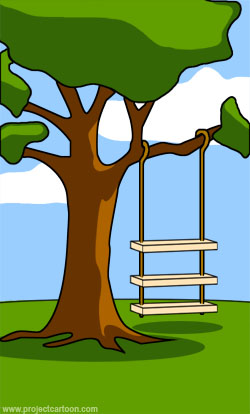
\includegraphics[width=1.0\textwidth]{./inf/SEKII/29_Softwaretechnik/PM_01.jpg}

Wie es der Kunde erklärt hat.
\end{center}
\end{minipage}
&
\begin{minipage}[t]{0.23\textwidth}
\begin{center}

\includegraphics[width=1.0\textwidth]{./inf/SEKII/29_Softwaretechnik/PM_02.jpg}

Wie es der Projekt-Manager verstanden hat.

\vspace*{3mm}
\end{center}
\end{minipage}
&
\begin{minipage}[t]{0.23\textwidth}
\begin{center}
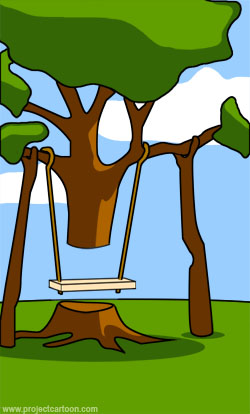
\includegraphics[width=1.0\textwidth]{./inf/SEKII/29_Softwaretechnik/PM_03.jpg}

Wie es der Analyst entworfen hat.
\end{center}
\end{minipage}
& 
\begin{minipage}[t]{0.23\textwidth}
\begin{center}

\includegraphics[width=1.0\textwidth]{./inf/SEKII/29_Softwaretechnik/PM_04.jpg}

Wie es programmiert wurde.
\end{center}
\end{minipage}
\\
\begin{minipage}[t]{0.23\textwidth}
\begin{center}
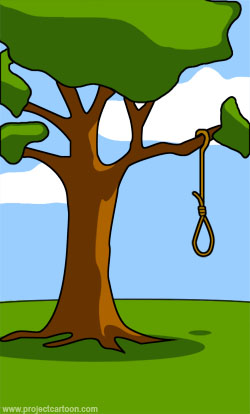
\includegraphics[width=1.0\textwidth]{./inf/SEKII/29_Softwaretechnik/PM_05.jpg}

Was die Beta-Tester bekommen haben.
\end{center}
\end{minipage}
&
\begin{minipage}[t]{0.23\textwidth}
\begin{center}
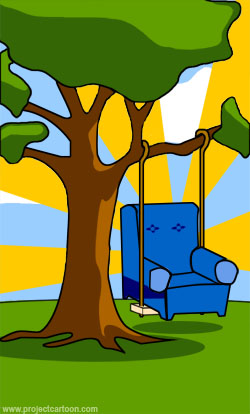
\includegraphics[width=1.0\textwidth]{./inf/SEKII/29_Softwaretechnik/PM_06.jpg}

Wie es der Business-Consultant beschrieben hat.

\vspace*{3mm}
\end{center}
\end{minipage}
& 
\begin{minipage}[t]{0.23\textwidth}
\begin{center}

\includegraphics[width=1.0\textwidth]{./inf/SEKII/29_Softwaretechnik/PM_07.jpg}

Wie das Projekt dokumentiert wurde.
\end{center}
\end{minipage}
&
\begin{minipage}[t]{0.23\textwidth}
\begin{center}

\includegraphics[width=1.0\textwidth]{./inf/SEKII/29_Softwaretechnik/PM_08.jpg}

Wie es supported wurde.
\end{center}
\end{minipage}
\\
\begin{minipage}[t]{0.23\textwidth}
\begin{center}
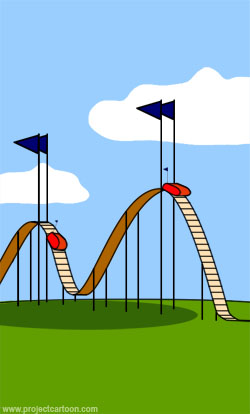
\includegraphics[width=1.0\textwidth]{./inf/SEKII/29_Softwaretechnik/PM_09.jpg}

Wie es dem Kunden in Rechnung gestellt wurde.
\end{center}
\end{minipage}
& 
\begin{minipage}[t]{0.23\textwidth}
\begin{center}
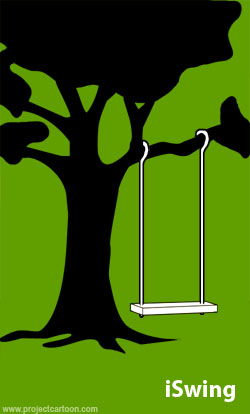
\includegraphics[width=1.0\textwidth]{./inf/SEKII/29_Softwaretechnik/PM_10.jpg}

Wie es vom Marketing beworben wurde.
\end{center}
\end{minipage}
& 
\begin{minipage}[t]{0.23\textwidth}
\begin{center}

\includegraphics[width=1.0\textwidth]{./inf/SEKII/29_Softwaretechnik/PM_11.jpg}

Wann es ausgeliefert wurde.
\end{center}
\end{minipage}
& 
\begin{minipage}[t]{0.23\textwidth}
\begin{center}
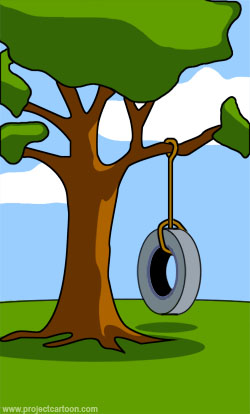
\includegraphics[width=1.0\textwidth]{./inf/SEKII/29_Softwaretechnik/PM_12.jpg}

Was der Kunde wirklich gebraucht hätte.
\end{center}
\end{minipage}
\\
\end{tabularx}
\egroup

\vspace{5mm}

Quelle: \url{http://projectcartoon.com/}